\chapter{Plugin Jenkins}

\section{Contexte initial}

Jenkins est le logiciel d'intégration continue, il utilisé à SAP dans le contexte des tests . Son rôle est d'intégrer les différents projets, tels que configuré par l'utilisateur, et met à disposition les résultats obtenus. Il permet d'avoir un retour régulier sur l'état des builds et du résultat de leurs tests.\\

Un plugin permettant une vision globale sur l'état des builds est déjà en place, Radiator. La figure \ref{figure:reportingPluginEnvironmentAfter} page \pageref{figure:reportingPluginEnvironmentAfter} présente son environnement d'utilisation. Nous pouvons y voir les développeurs et les ST qui alimentent le code hébergé sur Perforce que Jenkins l'utilise dans ses diverses intégrations. Au centre, le plugin permet un retour visuel rapide des livraisons Perforce.\\
Ce plugin est aussi conçu pour fonctionner avec un autre plugin, le plugin Claim. Il permet à quelqu'un visitant la page d'un job en échec de le \textquote{claimer}, inscrivant son identifiant ainsi qu'un message à destination de quiconque visiterai cette même page. Ceci permet de signaler que l'investigation est en cours.\\

\begin{figure}[!h]
  \centering
      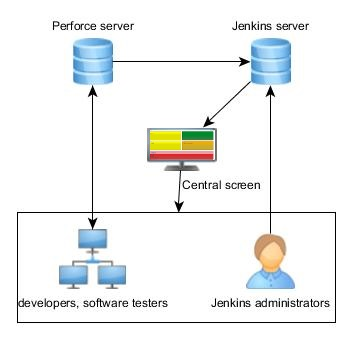
\includegraphics{images/reportingPluginEnvironmentAfter.jpg}
  \caption{L'environnement d'utilisation du plugin}
	\label{figure:reportingPluginEnvironmentAfter}
\end{figure}

Pour résumer ses caractéristiques principales, c'est un plugin qui permet :
\begin{itemize}
	\item d'afficher un écran  où chaque couleur correspond à un statut de build
	\item de rassembler les jobs par leurs préfixes communs
	\item de prendre en compte les claims
\end{itemize}

L'inconvénient est que le nombre de status existant ne permet pas la précision nécessaire pour définir l'état d'un jobs. Le plugin Radiator n'offre pas la malléabilité nécessaire. Voici la liste des différents états gérés par ce plugin : 
\begin{description}
	\item[SUCCESS] Le projet compile correctement et tous les tests sont passés
	\item[ABORTED] La compilation à été arrêtée en cours d'exécution
	\item[FAILURE] Le code ne compile pas
	\item[ERROR]
	\item[NOT BUILT] Le projet n'a pas été compilé
	\item[UNSTABLE] Des tests JUnit ne sont pas passés mais le code compile
	\item[CLAIM] Le job en échec à été claim par quelqu'un
\end{description}



Tel qu'il se présente le plugin ne permet pas de donner des informations autres que celles issues de Jenkins ou du plugin Claim. Il ne permet donc pas de donner de renseignements sur le defect associé à ce job. Tenir compte du defect permettrai de faire ressortir les régressions et autres erreurs, séparant ainsi les échecs pris en charge de ceux qui ne le sont pas.\\
Suite à la mission précédente nous avons maintenant accès aux informations relatives aux defects (celle-ci sont enregistrées dans les archives des builds sur le serveur Jenkins), dans un fichier XML que nous avons nommé test-defects (exemple page \pageref{testdefectxml}).\\



\textbf{La solution propos\'{e}e}\hfill \\ \indent
Dans un 1\up{er}, et en tant qu'exercice, il faudra réaliser un plugin offrant les mêmes possibilités d'affichage des builds. C'est-à-dire rassembler les jobs par préfixe et afficher le résultat général de tous ces groupes ainsi créés sur un unique écran. Ajouté aux caractéristiques, ce plugin doit pouvoir prendre en compte les informations du plugin Claim.\\ \indent
Dans un second temps, il faudra pouvoir ajouter un ou plusieurs statut(s) supplémentaire(s) ainsi que de ré-ajuster leur ordre de priorité. L'ajout de ce nouveau statuts doit être générique de sorte qu'un status quelconque puisse être ajouté.\\
Le plugin est donc capable de receuillir des informations dans des fichiers sans savoir, au préalable, comment seront structurées ses données. Rappelons que lors de l'exécution des tests, un fichier test-defect est généré contenant la liste\footnote{Au format xml} des jobs avec defect (exemple page \pageref{testdefectxml}).


\lstinputlisting[language=java,label=testdefectxml]{scripts/test-defects.xml}






\section{\'{E}tude préalable}
Les 1\up{er} impératifs ont été de maitraiser le langage et les outils qui me permettrai de mener ce projet à terme. Je n'avais jamais entendu parler de Jenkins ou d'un quelconque logiciel d'intégration continue, et a forciori sur la manière de l'étendre. 


Il existe un archétype maven (cf annexe \ref{annexe:maven} page \pageref{annexe:maven}) permettant de générer le squelette d'un plugin Jenkins\\

J'ai donc commencé par installer Jenkins et ses plugins, tels qu'ils sont utilisés à SAP, de manière à me familiariser avec ceux-ci. Pour examiner le comportementde Jenkins j'ai créé de faux projets me permettant de simuler les différents états possibles. Ceux-ci m'ont permis d'observer les différences entre les statuts Jenkins et JUnit, certains statuts portent les mêmes noms mais ne signifient pas les mêmes choses provoquent quelques incompréhensions. La signification de ces statuts étant l'objet de ce plugin, il m'incombai de les comprendre. Voici le détail des configurations que j'ai testé pour déterminer l'équivalence statut JUnit/statut Jenkins :

\begin{tabular}{|l|rr|c|c|}
	\hline
  \textbf{Description du projet} 							& \textbf{Status JUnit} 	& \textbf{Statut Jenkins}\\
  \hline
  projet vide et sans test 						& NA 						& Success\\
	
	projet vide et avec test réussi			& Passed				& Success\\
  
  projet vide avec test qui échoue 		& Failure				& Unstable\\
	
  projet avec erreur de compilation 	& NA						& Error\\
  \hline
\end{tabular}


Passée cette étape d'installations et de configurations je me suis penché sur la marche à suivre pour implémenter un plugin Jenkins.\\
La principale difficulté que j'ai eu à développer ce plugin a été de trouver l'information, il est reconnu sur internet que la documentation de Jenkins, lorsque l'on veut l'étendre, n'est pas clair. Mais la documentation officiel\footnote{\url{https://wiki.jenkins-ci.org/display/JENKINS/Extend+Jenkins}} offre un bel état des lieux de ce qu'il est possible de faire, décrit les différentes technologies constituant Jenkins et offre un tutoriel, trivial mais suffisant, pour comprendre les bases.\\



\section{Le 1\up{er} plugin}

Je me suis d'abord rendu sur la page du tutoriel officiel de Jenkins\footnote{\url{https://wiki.jenkins-ci.org/display/JENKINS/Plugin+tutorial}} afin d'obtenir un plugin fonctionnel avec lequel je pouvais faire mes expériences. Ensuite j'ai suivi un autre tutoriel\footnote{\url{https://cleantestcode.wordpress.com/2013/11/03/how-to-write-a-jenkins-plugin-part-1/}} non-officiel mais considérablement plus riche.\\

\subsection{Le squelette du plugin}
\subsubsection{Configuration}
D'après toutes les documentations disponible, le meilleur moyen de commencer le développement du plugin est d'utiliser maven\footnote{Maven 3 et JDK 6 ou plus récent} pour générer le squelette. Maven a besoin de configurations supplémentaires dans son settings.xml\footnote{Situé dans le répertoire \texttildelow/.m2} pour pouvoir récupérer les sources relatives à Jenkins.\\
Dans \textquote{pluginGroups} il faut ajouter la ligne suivante :
\begin{lstlisting}
<pluginGroup>org.jenkins-ci.tools</pluginGroup>
\end{lstlisting}
Et dans \textquote{profiles} il faut ajouter le profil suivant :
\begin{lstlisting}[language=xml]
<profile>
<id>jenkins</id>
<activation>
<activeByDefault>false</activeByDefault>
</activation>
<repositories>
<repository>
<id>repo.jenkins-ci.org</id>
<url>http://repo.jenkins-ci.org/public/</url>
</repository>
</repositories>
<pluginRepositories>
<pluginRepository>
<id>repo.jenkins-ci.org</id>
<url>http://repo.jenkins-ci.org/public/</url>
</pluginRepository>
</pluginRepositories>
</profile>
\end{lstlisting}

L'attribut de la balise \textquote{activeByDefault} est à false, parcequ'on travaille avec d'autres profils sur d'autres projet. Mais il faut retenir que ce paramètre peut empêcher la génération du squelette du plugin via la commande :
\begin{lstlisting}[language=xml]
mvn hpi:create
\end{lstlisting}

Pour exécuter cette commande ci-dessus il faut se placer dans le dossier qui recevra le projet. 


\subsubsection{Génération du squelette}
\`{A} l'exécution de cette commande il est demandé de renseigner le groupId et l'artifactId, le groupId peut être  org.jenkins-ci.plugins et l'artifactId est le nom du plugin. Cette commande crée l'arborescence du projet ainsi que les fichiers de base. 


\`{A} la génération du squelette du plugin nous obtenons un plugin qui compile dont l'architecture est présentée figure \ref{figure:hpiCreate} page \pageref{figure:hpiCreate}. Certaines choses importantes sont à notées, le pom.xml\footnote{Project Object Model} est généré à la base du projet dands lequel nous trouvons des informations telles que le parent de ce projet, les dépendances, l'auteur, la licence et la description.

\begin{figure}[!h]% h || ht || .... cf 
  \centering
      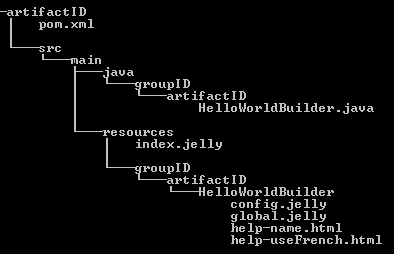
\includegraphics{images/hpiCreate.png}
  \caption{Architecture d'un plugin Jenkins généré par maven}
	\label{figure:hpiCreate}
\end{figure}
!!!!!! ok, maintenant on sais faire un plugin hello world

%\vspace{\stretch{1}}
Plusieurs autre fichiers sont générés :

\begin{tabular}{|l|p{0.7\linewidth}|}
  \hline
  \textbf{Nom du fichier} & \textbf{Description} \\
  \hline
  index.jelly & Description utilisée à la création d'une nouvelle instance du plugin \\
  config.jelly & Correspond à la page d'une instance du plugin \\
  global.jelly & Correspond à la page de configuration générale du plugin \\
  HelloWorldBuilder.java & Implémentation d'exemple du plugin \\
  help-name.html & Fichier d'aide à la configuration lorsque clic sur le symbole d'aide \\
  help-useFrench.html & Fichier d'aide à la configuration lorsque clic sur le symbole d'aide \\
  \hline
\end{tabular}


%\subsection{Architecture générique d'un plugin}


!!! Tous les fichiers
index.jelly
config.jelly
global.jelly

configure-entries.jelly
main.jelly
properties
help


!!!Les points d'extensions
\subsubsection{Déploiement du squelette du plugin}
Plusieurs solutions s'offre à nous pour déployer le plugin dans son environnement d'utilisation

\textbf{Installation \textquote{\`{a} la main}}\hfill \\ \indent 
En ligne de commande et depuis la racine du projet\footnote{\`{a} l'emplacement du POM.xml}, il faut exécuter la commande suivante :
\begin{lstlisting}
mvn clean install -Pjenkins
\end{lstlisting}
Celle-ci va télécharger les sources nécessaires, les compiler, exécuter les tests et, si tout se passe bien, générer le fichier .hpi dans le dossier target.\\
Ceci fait, il faut se rendre dans Jenkins (par exemple http://localhost:8080/ ou autre. En fonction de la configuration), s'identifier et aller dans les paramètres avancés de gestion de plugins. Ici il faut renseigner le chemin d'accès vers le .hpi et terminer.\\


\textbf{Commande du plugin Jenkins de maven}\hfill \\ \indent 
En ligne de commande et depuis la racine du projet, il faut exécuter la commande suivante :
\begin{lstlisting}
mvn hpi:run -Djetty.port=8090 -Pjenkins
\end{lstlisting}
Cette commande va déployer une instances de Jenkins propre à maven, ce qui nous permet d'exécuter le plugin ainsi que de le debugger. On peut très bien omettre de préciser le port utilisé si celui par défaut\footnote{port 8080} est disponible, mais il vaut mieux éviter. Une fois que le déploiement est terminé maven signale que \textquote{Jenkins is fully up and running} nous pouvons aller voir Jenkins à l'url \emph{http://localhost:8080/jenkins} qui devrait ressembler à la figure \ref{figure:firstJenkinsWhenGenerateTheSkeletonPlugin} page \pageref{figure:firstJenkinsWhenGenerateTheSkeletonPlugin}.
\begin{figure}[!h]
  \centering
      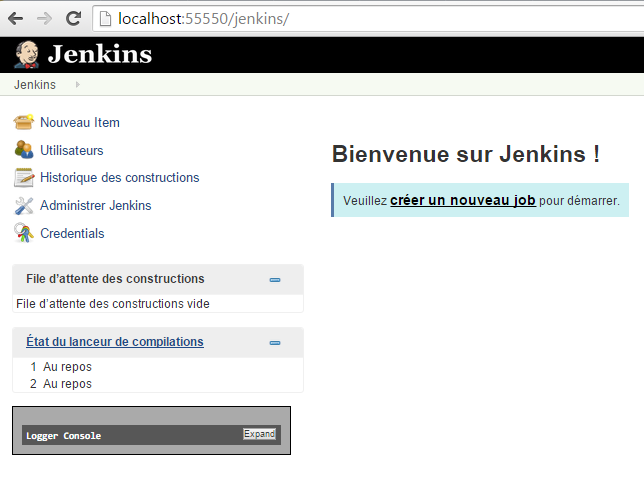
\includegraphics[width=\textwidth]{images/firstJenkinsWhenGenerateTheSkeletonPlugin.png}
  \caption{Jenkins à l'exécution de la commande maven qui l'encapsule}
	\label{figure:firstJenkinsWhenGenerateTheSkeletonPlugin}
\end{figure}



\subsubsection{Essaie du squelette du plugin}
Jenkins se redémarre et voilà notre plugin intégré à celui-ci. Nous pouvons aller voir l'écran de configuration générale vérifier que le fichier global.jelly a bien été ajouté, on coche la case. Maintenant configurons un projet au hasard et ajoutons une étape pré build, nous aperçevons un item s'appelant \textquote{say hello world}, essayons et remplissons le champ de texte. Compilons le projet et regardons la sortie console, au début nous voyons affiché notre texte.\\
Nous avons donc un plugin qui permet de dire quelque chose en début ou fin de build. 



\section{Implémentation de la base du nouveau plugin}

Nous avons donc un plugin qui étend le comportement lors des builds que Jenkins exécute, ceci grâce au point d'extension Builder.\\
Jenkins possède beaucoup de points d'extensions et à cette étape il faut déterminer lequel, ainsi que quelle classe étendre! Dans le cas où aucun point d'extension ne correspond, il est très facile d'en créer un en suivant la documention. Autrement, nous pouvons nous inspirer du plugin Radiator est regarder quelle classe il étend.\\
En parcourant la liste des points d'extensions disponibles nous pouvons trouver \emph{View}, dont l'une de ses implémentation est \emph{ListView}; sa description étant \textquote{Displays Jobs in a flat list view}. Notre objectif étant d'afficher les Jobs, cette solution semble correspondre. De plus, en observant la javadoc on peut trouver la méthode nous donnant accès aux projet associés à la vue (figure \ref{figure:listviewJavaDoc} page \pageref{figure:listviewJavaDoc}).

\begin{figure}[!h]
  \centering
      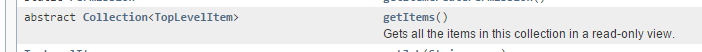
\includegraphics[width=\textwidth]{images/listviewJavaDoc.png}
  \caption{Extrait de la javadoc de la classe ListView}
	\label{figure:listviewJavaDoc}
\end{figure}



\subsection{Import du code dans l'IDE}
J'ai expérimenté deux IDE pour développer le plugin : Eclipse puis NetBeans.\\
En utilisant Eclipse j'ai rencontré beaucoup de problèmes liés aux configurations maven et d'Eclipse, de telle sorte qu'à un certain moment je me trouvais obligé de compiler le code via Jenkins, de récupérer le .hpi en local pour l'intégrer ensuite à Jenkins!
Le cycle de développement était le suivant :

\begin{enumerate}
	\item Implémentation du code sous Eclipse
	\item Compilation du code grâce à maven (ou Jenkins!) et génération du fichier .hpi
	\item Désinstallation du plugin de Jenkins + redémarrage
	\item Installation du nouveau plugin sur Jenkins + redémarrage
	\item Test du plugin
\end{enumerate}
L'utilisation de Netbeans (et de son plugin Jenkins) évite de passer par toutes ses étapes car il suffit de cliquer sur run pour exécuter le plugin et sur debug pour le debugger. Cela facilite l'implémentation du code et, surtout, permet de se focaliser sur les problèmes liés au plugin plutôt qu'à ceux liés aux outils de développement.\\


\subsection{Implémentation de la base}

Avant de pouvoir vraiment travailler à l'implémentation des fonctionnalités du logiciel il faut encore savoir où écrire le code et comment nommer ses fichier. Une fois que Jenkins à localiser l'annotation précisant qu'il s'agit d'un plugin, il utilise une convention de nommage pour accéder aux différents fichiers d'aide ou de configuration. Pour savoir comment doit se nommer mon fichier de configuration je vais chercher où, dans jenkins-core, se trouve les fichiers de configuration de Listview. Ce qui me m'offrira la possiblité d'implémenter ma propre configuration. L'arborescence de ce fichier est illustrée figure \ref{figure:listviewJavaDoc} page \pageref{figure:listviewJavaDoc}. Il convient maintenant de copier ce fichier et de le coller dans le répertoire \emph{ressources} de notre projet.


\begin{figure}[!h]
  \centering
      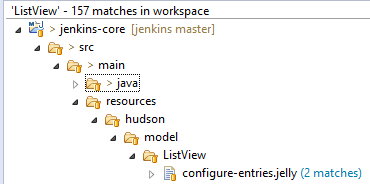
\includegraphics{images/listviewSearch.png}
  \caption{Chemin d'accès au fichier de configuration par défaut}
	\label{figure:listviewSearch}
\end{figure}

Maintenant que l'on peut personnaliser la configuration du plugin, il faut pouvoir faire de même avec l'affichage de la vue. Nous allons donc créer un nouveau fichier \emph{main.xml} qui contiendra le code de l'interface graphique du plugin.\\

Après quelques tests rapides on s'aperçois que beaucoup de code, css ou JavaScript, est exécuté lorsque l'on accède à la page. Il faut donc réinitialiser pour travailler dans de bonnes conditions. Premièrement, on supprime l'affichage du header, footer et side-panel de Jenkins (cf figure \ref{figure:cssInit} page \pageref{figure:cssInit}) et deuxièment on supprime l'affichage du side-panel, après chargement de la page (cf figure \ref{figure:cssInitJS} page \pageref{figure:cssInitJS}).\\

\begin{figure}[!h]
  \centering
      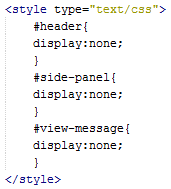
\includegraphics{images/cssInit.png}
  \caption{Initialisation des css avant chargement}
	\label{figure:cssInit}
\end{figure}

\begin{figure}[!h]
  \centering
      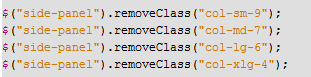
\includegraphics{images/cssInitJS.png}
  \caption{Initialisation des css après chargement}
	\label{figure:cssInitJS}
\end{figure}


\section{Travail réalisé}




\begin{figure}[!h]
  \centering
      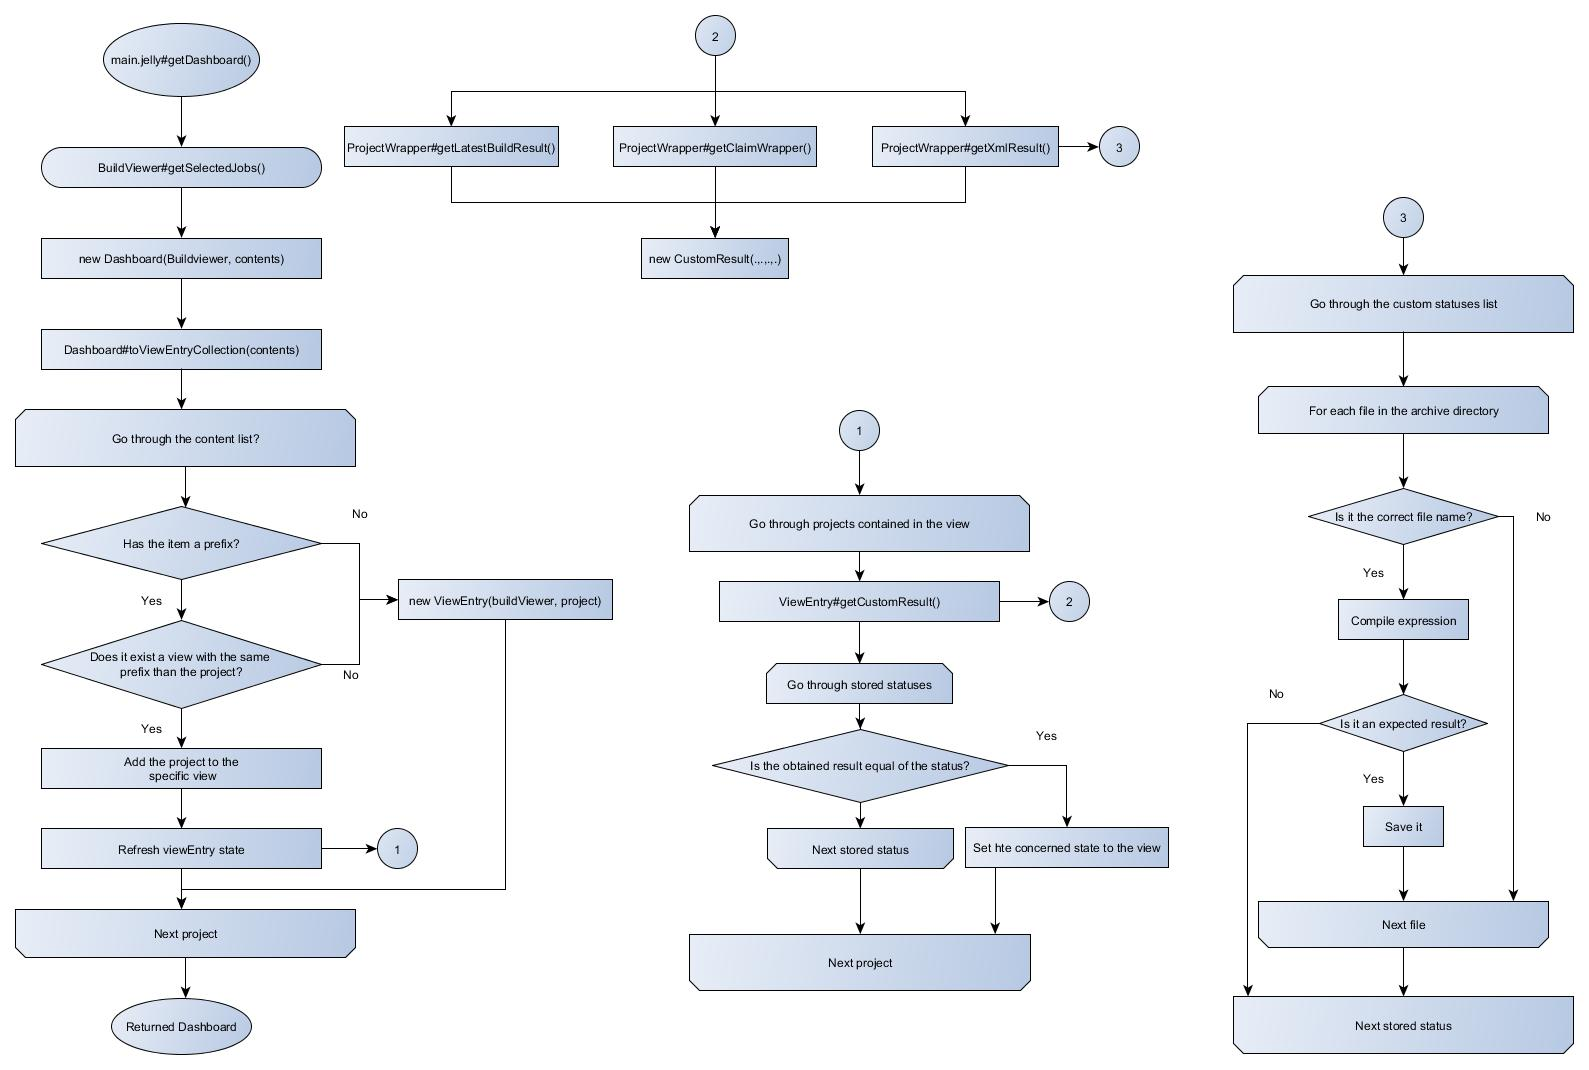
\includegraphics[width=\textheight,angle=90]{images/dashboardGenesis.jpg}
  \caption{Algorithme de création du Dashboard}
	\label{figure:dashboardGenesis}
\end{figure}


\begin{figure}[!h]
  \centering
      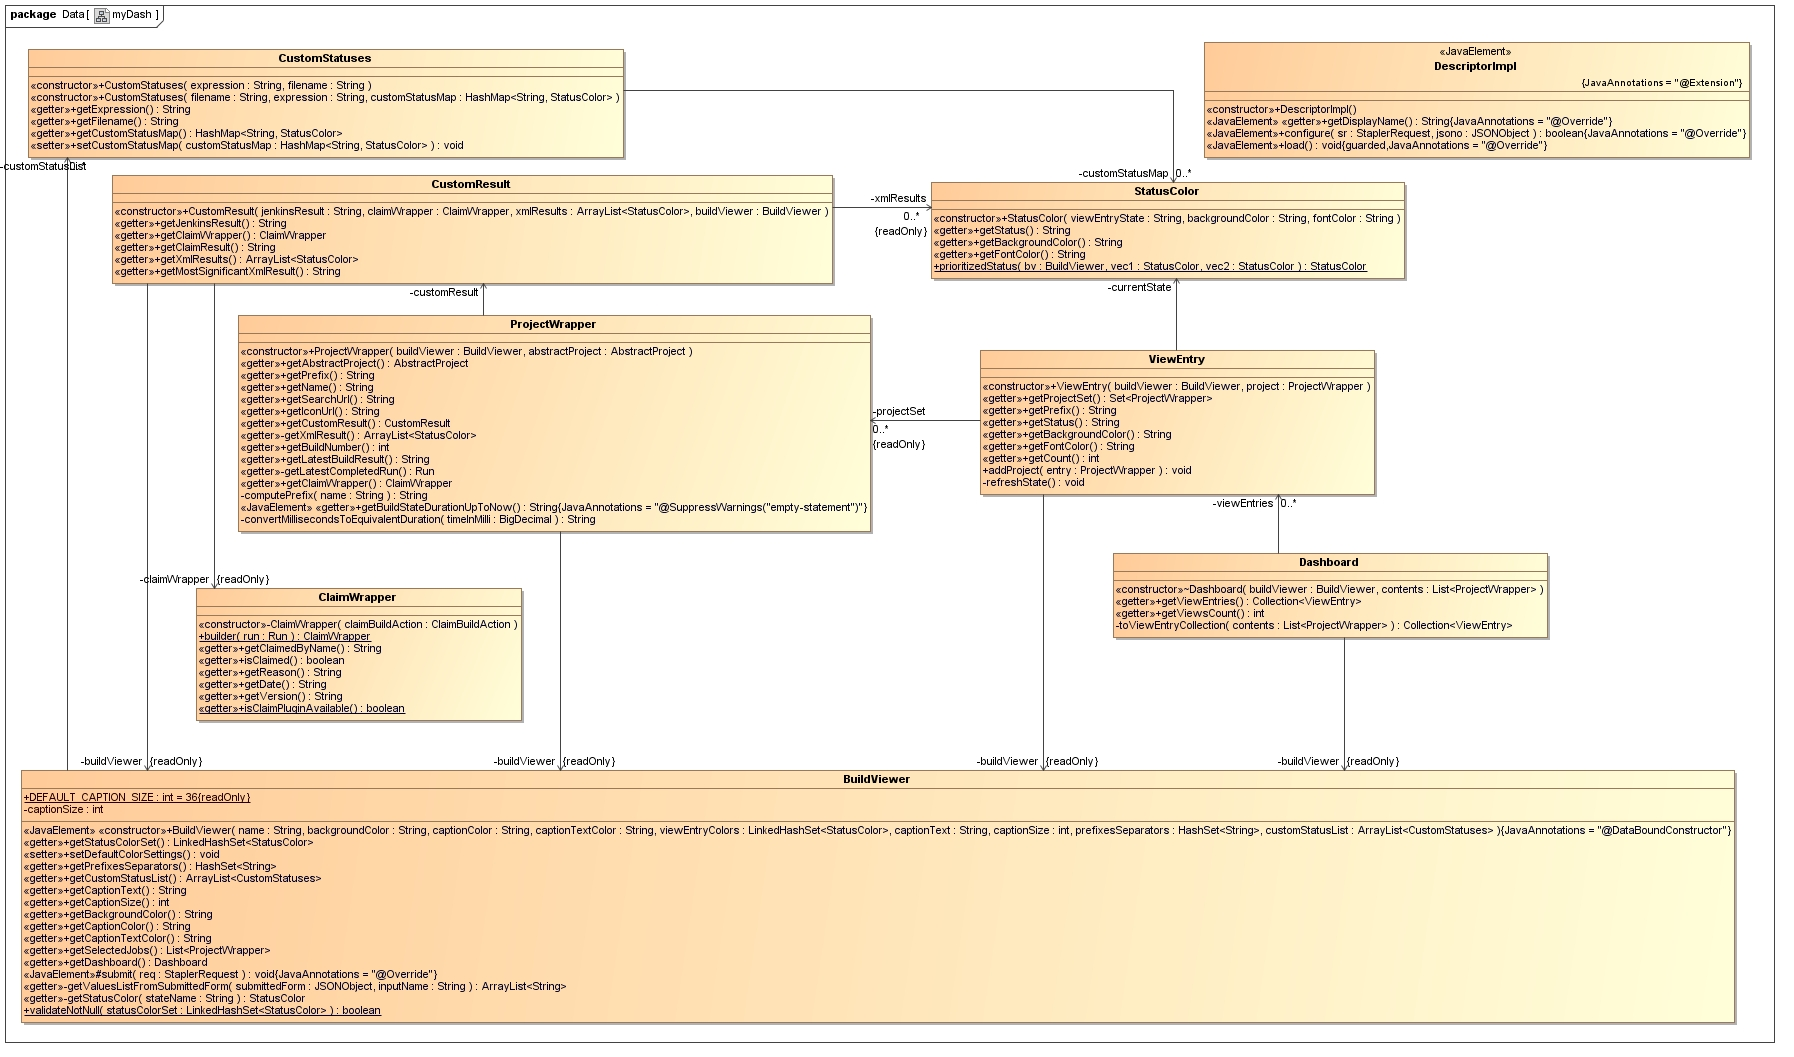
\includegraphics[width=\textheight,angle=90]{images/myDash.jpg}
  \caption{Diagramme de classe du plugin réalisé}
	\label{figure:myDash}
\end{figure}
